\documentclass[a4paper, 12pt]{article}
% packages
\usepackage{amssymb}
\usepackage[fleqn]{mathtools}
\usepackage{tikz}
\usepackage{enumerate}
\usepackage{bussproofs}
\usepackage{xcolor}
\usepackage[margin=1.3cm]{geometry}
\usepackage{logicproof}
\usepackage{diagbox}
\usepackage{listings}
\usepackage{graphicx}
\usepackage{lstautogobble}
\usepackage{hyperref}
\usepackage{multirow}
\usepackage{tipa}
\usetikzlibrary{decorations.pathreplacing, arrows, shapes.gates.logic.US, circuits.logic.US, calc, automata, positioning, intersections}

\allowdisplaybreaks

% shorthand for verbatim
% this clashes with logicproof, so maybe fix this at some point?
\catcode`~=\active
\def~#1~{\texttt{#1}}

% code listing
\lstdefinestyle{main}{
    numberstyle=\tiny,
    breaklines=true,
    showspaces=false,
    showstringspaces=false,
    tabsize=2,
    numbers=left,
    basicstyle=\ttfamily,
    columns=fixed,
    fontadjust=true,
    basewidth=0.5em,
    autogobble,
    xleftmargin=3.0ex,
    mathescape=true
}
\newcommand{\dollar}{\mbox{\textdollar}} %
\lstset{style=main}

% augmented matrix
\makeatletter
\renewcommand*\env@matrix[1][*\c@MaxMatrixCols c]{%
\hskip -\arraycolsep
\let\@ifnextchar\new@ifnextchar
\array{#1}}
\makeatother

% ceiling / floor
\DeclarePairedDelimiter{\ceil}{\lceil}{\rceil}
\DeclarePairedDelimiter{\floor}{\lfloor}{\rfloor}

% custom commands
\newcommand{\indefint}[2]{\int #1 \, \mathrm{d}#2}
\newcommand{\defint}[4]{\int_{#1}^{#2} #3 \, \mathrm{d}#4}
\newcommand{\pdif}[2]{\frac{\partial #1}{\partial #2}}
\newcommand{\dif}[2]{\frac{\mathrm{d}#1}{\mathrm{d}#2}}
\newcommand{\limit}[2]{\raisebox{0.5ex}{\scalebox{0.8}{$\displaystyle{\lim_{#1 \to #2}}$}}}
\newcommand{\summation}[2]{\sum\limits_{#1}^{#2}}
\newcommand{\product}[2]{\prod\limits_{#1}^{#2}}
\newcommand{\intbracket}[3]{\left[#3\right]_{#1}^{#2}}
\newcommand{\ulsmash}[1]{\underline{\smash{#1}}}

\newcommand{\powerset}[0]{\wp}
\renewcommand{\emptyset}[0]{\varnothing}

\makeatletter
\newsavebox{\@brx}
\newcommand{\llangle}[1][]{\savebox{\@brx}{\(\m@th{#1\langle}\)}%
  \mathopen{\copy\@brx\kern-0.5\wd\@brx\usebox{\@brx}}}
\newcommand{\rrangle}[1][]{\savebox{\@brx}{\(\m@th{#1\rangle}\)}%
  \mathclose{\copy\@brx\kern-0.5\wd\@brx\usebox{\@brx}}}
\makeatother
\newcommand{\lla}{\llangle}
\newcommand{\rra}{\rrangle}
\newcommand{\la}{\langle}
\newcommand{\ra}{\rangle}
\newcommand{\crnr}[1]{\text{\textopencorner} #1 \text{\textcorner}}
\newcommand{\laplace}{\mathcal{L}}
\newcommand{\fourier}{\mathcal{F}}

\newcommand{\mat}[1]{\boldsymbol{#1}}
\renewcommand{\vec}[1]{\boldsymbol{#1}}
\newcommand{\rowt}[1]{\begin{bmatrix}
    #1
\end{bmatrix}^\top}

\newcommand{\unaryproof}[2]{\AxiomC{#1} \UnaryInfC{#2} \DisplayProof}
\newcommand{\binaryproof}[3]{\AxiomC{#1} \AxiomC{#2} \BinaryInfC{#3} \DisplayProof}
\newcommand{\trinaryproof}[4]{\AxiomC{#1} \AxiomC{#2} \AxiomC{#3} \TrinaryInfC{#4} \DisplayProof}

\newcommand{\axiom}[1]{\AxiomC{#1}}
\newcommand{\unary}[1]{\UnaryInfC{#1}}
\newcommand{\binary}[1]{\BinaryInfC{#1}}
\newcommand{\trinary}[1]{\TrinaryInfC{#1}}
\newcommand{\quaternary}[1]{\QuaternaryInfC{#1}}
\newcommand{\quinary}[1]{\QuinaryInfC{#1}}
\newcommand{\dproof}[0]{\DisplayProof}

\newcommand{\bnfsep}[0]{\ |\ }
\newcommand{\lrbt}[0]{\ \bullet\ }
\newcommand{\concsep}[0]{\ ||\ }
\newcommand{\ttbs}{\char`\\}

\newcommand{\violet}[1]{\textcolor{violet}{#1}}
\newcommand{\blue}[1]{\textcolor{blue}{#1}}
\newcommand{\red}[1]{\textcolor{red}{#1}}

% no indent
\setlength\parindent{0pt}

% reasoning proofs
\usepackage{ltablex}
\usepackage{environ}
\keepXColumns
\NewEnviron{reasoning}{
    \begin{tabularx}{\textwidth}{rlX}
        \BODY
    \end{tabularx}
}
\newcommand{\proofline}[3]{$(#1)$ & $#2$ & \hfill #3 \smallskip \\}
\newcommand{\proofarbitrary}[1]{& take arbitrary $#1$ \smallskip \\}
\newcommand{\prooftext}[1]{\multicolumn{3}{l}{#1} \smallskip \\}
\newcommand{\proofmath}[3]{$#1$ & = $#2$ & \hfill #3 \smallskip \\}
\newcommand{\prooftherefore}[1]{& $\therefore #1$ \smallskip \\}
\newcommand{\proofbc}[0]{\prooftext{\textbf{Base Case}}}
\newcommand{\proofis}[0]{\prooftext{\textbf{Inductive Step}}}

% reasoning er diagrams
\newcommand{\nattribute}[4]{
    \node[draw, state, inner sep=0cm, minimum size=0.2cm, label=#3:{#4}] (#1) at (#2) {};
}
\newcommand{\mattribute}[4]{
    \node[draw, state, accepting, inner sep=0cm, minimum size=0.2cm, label=#3:{#4}] (#1) at (#2) {};
}
\newcommand{\dattribute}[4]{
    \node[draw, state, dashed, inner sep=0cm, minimum size=0.2cm, label=#3:{#4}] (#1) at (#2) {};
}
\newcommand{\entity}[3]{
    \node[] (#1-c) at (#2) {#3};
    \node[inner sep=0cm] (#1-l) at ($(#1-c) + (-1, 0)$) {};
    \node[inner sep=0cm] (#1-r) at ($(#1-c) + (1, 0)$) {};
    \node[inner sep=0cm] (#1-u) at ($(#1-c) + (0, 0.5)$) {};
    \node[inner sep=0cm] (#1-d) at ($(#1-c) + (0, -0.5)$) {};
    \draw
    ($(#1-c) + (-1, 0.5)$) -- ($(#1-c) + (1, 0.5)$) -- ($(#1-c) + (1, -0.5)$) -- ($(#1-c) + (-1, -0.5)$) -- cycle;
}
\newcommand{\relationship}[3]{
    \node[] (#1-c) at (#2) {#3};
    \node[inner sep=0cm] (#1-l) at ($(#1-c) + (-1, 0)$) {};
    \node[inner sep=0cm] (#1-r) at ($(#1-c) + (1, 0)$) {};
    \node[inner sep=0cm] (#1-u) at ($(#1-c) + (0, 1)$) {};
    \node[inner sep=0cm] (#1-d) at ($(#1-c) + (0, -1)$) {};
    \draw
    ($(#1-c) + (-1, 0)$) -- ($(#1-c) + (0, 1)$) -- ($(#1-c) + (1, 0)$) -- ($(#1-c) + (0, -1)$) -- cycle;
}

% actual document
\begin{document}
    \section*{CO245 - Probability and Statistics}
        \subsection*{15th January 2020}
            Probability is a mathematical formalism used to describe and quantify uncertainty.
            \subsubsection*{Sample Spaces and Events}
                \begin{itemize}
                    \itemsep0em
                    \item \textbf{sample space} \hfill $S$ or $\Omega$
                        \subitem a set containing the possible outcomes of a random experiment
                        \subitem for example; sample space of two coin tosses \hfill $S = \{ (H, H), (H, T), (T, H), (T, T)\}$
                    \item \textbf{event} \hfill $E$ ($E \subseteq S$)
                        \subitem any subset of the sample space (collection of some possible events)
                        \subitem for example; event of the first coin being heads in two tosses \hfill $E = \{ (H, H), (H, T) \}$
                        \subitem the extremes are $\emptyset$ (the null event) which will never occur, or $S$ (the universal event) which will always occur - there is only uncertainty when the events are strictly between the events, such that $\emptyset \subset E \subset S$
                    \item \textbf{elementary event} \hfill singleton subset containing exactly one element from $S$
                \end{itemize}
                When performing a random experiment, the outcome will be a single element $s^* \in S$.
                Then an event $E \subseteq S$ has \textbf{occurred} iff $s^* \in E$.
                If it has not occurred, then $s^* \notin E \Leftrightarrow s^* \in \bar{E}$ (can be read as not $E$).
                \medskip

                With a set of events $\{ E_1, E_2, \dots \}$, we can have the following set operations;
                \begin{itemize}
                    \itemsep0em
                    \item $\bigcup\limits_i E_i = \{ s \in S \bnfsep \exists i.\ [s \in E_i] \}$ \hfill will only occur if at least one of the events $E_i$ occurs ("or")
                    \item $\bigcap\limits_i E_i = \{ s \in S \bnfsep \forall i.\ [s \in E_i] \}$ \hfill will only occur if all of the events $E_i$ occurs ("and")
                    \item $\forall i, j.\ E_i \cap E_j = \emptyset$ \hfill ($i \neq j$) if they are mutually exclusive (at most one can occur)
                \end{itemize}
            \subsubsection*{$\sigma$-algebra}
                In an uncountably infinite set, the event set you are assigning probabilities to cannot be every subset, as the probabilities cannot be made to sum to 1 under reasonable axioms.
                \medskip

                We define the $\sigma$-algebra as the subset of events which we can assign probabilities to.
                We want to define a probability function $P$ that corresponds to the subsets of $S$ that we wish to \textbf{measure}.
                This set of subsets is referred to as $\mathfrak{S}$ (the event space), with the following three properties (corresponding to the axioms of probability);
                \begin{itemize}
                    \itemsep0em
                    \item nonempty \hfill $S \in \mathfrak{S}$
                    \item closed under complements \hfill $E \in \mathfrak{S} \Rightarrow \bar{E} \in \mathfrak{S}$
                    \item closed under countable union (therefore any countable set is fine) \hfill $E_1, E_2, \dots \in \mathfrak{S} \Rightarrow \bigcup\limits_i E_i \in \mathfrak{S}$
                \end{itemize}
                A probability measure on the pair $(S, \mathfrak{S})$ is a mapping $P : \mathfrak{S} \to [0, 1]$, satisfying the following three axioms;
                \begin{itemize}
                    \itemsep0em
                    \item $\forall E \in \mathfrak{S}.\ [0 \leq P(E) \leq 1]$
                    \item $P(S) = 1$
                    \item countably additive, for \textbf{disjoint subsets} $E_1, E_2, \dots \in \mathfrak{S}$ \hfill $P\left(\bigcup\limits_i E_i\right) = \summation{i}{} P(E_i)$
                \end{itemize}
                From these, we can derive the following;
                \begin{itemize}
                    \itemsep0em
                    \item $P(\bar{E}) = 1 - P(E)$
                        $$\underbrace{P(E) + P(E)}_\text{disjoint} = P(\underbrace{E \cup \bar{E}}_{E \cup \bar{E} = S}) = P(S) = 1$$
                    \item $P(\emptyset) = 0$ \hfill special case of the above, when $E = S$
                    \item for any events $E$ and $F$ \hfill $P(E \cup F) = P(E) + P(F) - P(E \cap F)$
                \end{itemize}
        \subsection*{16th January 2020}
            \subsubsection*{Independent Events}
                It's important to note that independent events are \textbf{not} the same as disjoint events.
                Two events $E$ and $F$ are independent iff $P(E \cap F) = P(E) P(F)$ - sometimes written as $E \perp F$.
                Generally, a set of events $\{ E_1, E_2, \dots \}$ are set to be independent if for any finite subset $\{ E_{i_1}, E_{i_2}, \dots, E_{i_n} \}$;
                $$P\left(\bigcap\limits_{j = 1}^n E_{i_j}\right) = \product{j = 1}{n}P(E_{i_j})$$
                Where we have $\{ i_j \bnfsep 1 \leq j \leq n \}$ is any set of distinct positive integers.
                Note that independence is more than just pairwise independence.
                \medskip

                We propose that if events $E$ and $F$ are independent, then $\bar{E}$ and $F$ are also independent.
                Note that $E$ and $\bar{E}$ form a partition of $S$ (they are disjoint, and union to $S$).
                $F = (E \cap F) \cup (\bar{E} \cap F)$ is a disjoint union (and also a partition of $F$), this gives us $P(F) = P(E \cap F) + P(\bar{E} \cap F) \Rightarrow P(\bar{E} \cap F) = P(F) - P(E \cap F)$;
                \begin{align*}
                    P(\bar{E} \cap F) & = P(F) - P(E \cap F) & \text{$E$ and $F$ are independent}, \Rightarrow \\
                    & = P(F) - P(E) P(F) & \Rightarrow \\
                    & = (1 - P(E))P(F) & \text{probability of complement}, \Rightarrow \\
                    & = P(\bar{E}) P(F) & \text{hence independent}, \blacksquare
                \end{align*}
            \subsubsection*{Interpretations of Probability}
                In order to assign meaning to $P$, we need to have some interpretation of probability, such as the following;
                \begin{itemize}
                    \itemsep0em
                    \item \textbf{classical}
                        \medskip

                        If $S$ is finite, and the elementary events are "equally likely", then for an event $E \subseteq S$, the probability is the number of outcomes in $E$ out of the total number of possible outcomes ($S$);
                        $$P(E) = \frac{| E |}{| S |}$$
                        This idea of "equally likely" (uniform) can be extended to infinite spaces.
                        Instead of taking the set cardinality, another standard measure (such as area or volume) can be used instead.
                    \item \textbf{frequentist}
                        \medskip

                        The idea is that if someone were to perform the same experiment ($E$ may or may not occur) in identical random situations many times, then the proportion of times $E$ occurs will tend to some limiting value, which would be $P(E)$.
                    \item \textbf{subjective}
                        \medskip

                        Not assessed.
                        Probability is the degree of belief held by an individual (see \textit{De Finetti}) - suppose a random event $E \subseteq S$ is to be performed, and an individual enters a game regarding this experiment, with two choices;
                        \begin{itemize}
                            \itemsep0em
                            \item gamble \hfill if $E$ occurs they win \$1, otherwise if $\bar{E}$ occurs they win \$0
                            \item stick \hfill regardless of the outcome, the individual receives \$$P(E)$
                        \end{itemize}
                        The critical value of $P(E)$, where the individual is indifferent between the choices, is their probability of $E$.
                \end{itemize}
            \subsubsection*{Dependent Probabilities and Conditional Probability}
                For the standard example of flipping a coin and rolling a die (assuming both fair), we have independence - the probability of each elementary event is $\frac{1}{2} \cdot \frac{1}{6} = \frac{1}{12}$.
                \medskip

                However, consider the case where we have two die, where the first is fair, and the second is a "top", where we only have odd numbers (such that a roll of a 2 is mapped to a 5, 4 to 3, and 6 to 1).
                When we now flip the coin, if it is heads, we use the normal die, otherwise if it is tails, we use the "top".
                As expected, this is no longer independent.
                \medskip

                For two events $E$ and $F$ in $S$, where $P(F) \neq 0$, we can define the probability of $E$ occurring, given that we know $F$ has occurred to be;
                $$P(E|F) = \frac{P(E \cap F)}{P(F)}$$
                Note that this also holds for independence ($P(E)$ doesn't change, as expected);
                $$P(E|F) = \frac{P(E \cap F)}{P(F)} = \frac{P(E) P(F)}{P(F)} = P(E)$$
                An example of this is as follows - suppose we roll two normal dice, with one from each hand.
                The sample space is all the ordered pairs of possible values $S = \{ (1, 1), (1, 2), \dots, (6, 6) \}$.
                Let the event $E$ be defined as the die from the left hand has a higher value than the die from the right hand.
                Looking at all possible combinations, we have;
                $$P(E) = \frac{15}{36}$$
                Suppose we now know $F$, the value of the left die being 5, has occurred.
                Since we know $F$ has occurred, the only events that could have happened are $F = \{ (5, 1), (5, 2), \dots, (5, 6) \}$.
                Similarly, the only sample space elements in $E$ that could've occurred are $E \cap F = \{ (5, 1), (5, 2), (5, 3), (5, 4) \}$.
                Our probability is as follows;
                $$\frac{| E \cap F |}{| F |} = \frac{4}{6} = \frac{\frac{4}{36}}{\frac{1}{6}} = \frac{P(E \cap F)}{P(F)} \equiv P(E|F)$$

                One way to think about probability conditioning as a shrinking of the sample space, with events being replaced by intersections with the reduced space, and a rescaling of the probabilities.
                For example, with $F = S$, we have the following;
                $$P(E) = \frac{P(E)}{1} = \frac{P(E \cap S)}{P(S)} = P(E|S)$$
                Furthermore, we can extend the idea of independence of events with respect to a probability measure $P$ to conditional probabilities.
                $P(\cdot |F)$ is a valid probability measure which obeys the axioms of probability on the set $F$.
                For three events $E_1, E_2, F$, the event pair $E_1$ and $E_2$ are conditionally independent given $F$ (sometimes written as $E_1 \bot E_2|F$) if and only if;
                \begin{center}
                    $P(E_1 \cap E_2 | F) = P(E_1|F) P(E_2|F)$
                \end{center}
            \subsubsection*{Bayes Theorem}
                For two events $E$ and $F$ in $S$, we have $P(E \cap F) = P(F) P(E|F)$, and $P(E \cap F) = P(E) P(F|E)$ (interchanging, and noting commutativity of $\cap$).
                Hence we have Bayes Theorem;
                $$P(E|F) = \frac{P(E) P(F|E)}{P(F)}$$
            \subsubsection*{Partition Rule}
                Consider a set of events $\{ F_1, F_2, \dots \}$, which form a partition of $S$ (they are disjoint, and union together to form $S$).
                Then for any event $E \subseteq S$, the partition rule states;
                $$P(E) = \summation{i}{} P(E|F_i) P(F_i)$$
                The proof is as follows;
                \begin{align*}
                    E & = E \cap S \\
                    & = E \cap \bigcup\limits_i F_i & \text{by definition of partitions} \\
                    & = \bigcup\limits_i (E \cap F_i) & \text{by distributivity of intersection} \\
                    P(E) & = P\left(\bigcup\limits_i (E \cap F_i)\right) \\
                    & = \summation{i}{} P(E \cap F_i) & \text{disjoint union} \\
                    & = \summation{i}{} P(E|F_i) P(F_i)
                \end{align*}
                Note that $\{ E \cap F_1, E \cap F_2, \dots \}$ is disjoint if $\{ F_1, F_2, \dots \}$ is.
                Assume there is an element $s \in E \cap F_i$ and $s \in E \cap F_j$ (where $i \neq j$), if it is in both, then $s \in F_i$ and $s \in F_j$, which is not possible.
                \medskip

                Note that $\{ F, \bar{F} \}$ forms a partition of $S$, therefore by the Law of Total Probability we have;
                \begin{center}
                    $P(E) = P(E \cap F) + P(E \cap \bar{F}) = P(E|F) P(F) + P(E|\bar{F}) P(\bar{F})$
                \end{center}
            \subsubsection*{Terminology}
                \begin{itemize}
                    \itemsep0em
                    \item conditional probabilities \hfill $P(E|F)$
                    \item joint probabilities \hfill $P(E \cap F)$
                    \item marginal probabilities (margins of a table) \hfill $P(E)$
                        \subitem margins of a table
                \end{itemize}
            \subsubsection*{Likelihood and Posterior Probability}
                Suppose we have a probability model with parameters $\theta$, that define a model instance (such as $\mu$ and $\sigma$), and a set of observations (or evidence) $X$.
                \begin{itemize}
                    \itemsep0em
                    \item \textbf{likelihood function} (probability of the evidence, given  the parameters) \hfill $P(X|\theta)$
                        \subitem what is the probability our model will predict that evidence?
                    \item \textbf{posterior probability} (probability of the parameters, given the evidence) \hfill $P(\theta|X)$
                        \subitem what is the probability the actual parameters are $\theta$, given our evidence?
                    \item \textbf{prior probability} (not taking into account the evidence) \hfill $P(\theta)$
                \end{itemize}
                This is related by Bayes theorem;
                $$P(\theta|X) = \frac{P(X|\theta) P(\theta)}{P(X)}$$
                \begin{center}
                    posterior probability $\propto$ likelihood $\times$ prior probability
                \end{center}
                This is then divided by the normalising constant;
                $$\summation{\theta}{} P(X|\theta) P(\theta) = P(X)$$
        \subsection*{22nd January 2020}
            \subsubsection*{Example Questions}
                \begin{enumerate}[1.]
                    \itemsep0em
                    \item
                        There are 5000 VLSI chips, 1000 from company $X$ (which has a 10\% chance of being defective), and 4000 from company $Y$ (which has a 5\% chance of being defective).
                        If a chip is defective, what is the probability it came from company $X$?
                        \medskip

                        Let $E$ be the event that the randomly selected chip was made by $X$, and $F$ be the event that the chip is defective.
                        \begin{align*}
                            P(E) & = \frac{1000}{5000} \\
                            & = 0.2 \\
                            P(\bar{E}) & = \frac{4000}{5000} \\
                            & = 0.8 \\
                            P(F|E) & = 0.1 & \text{given} \\
                            P(F|\bar{E}) & = 0.05 & \text{given} \\
                            P(E \cap F) & = P(F|E) P(E) \\
                            & = 0.02 \\
                            P(\bar{E} \cap F) & = P(F|\bar{E}) P(\bar{E}) \\
                            & = 0.04
                        \end{align*}
                        This gives us enough to fill in the table, as well as the \violet{missing entries} with the law of total probabilities;
                        \begin{center}
                            \begin{tabular}{c|cc|c}
                                & $E$ & $\bar{E}$ & \\
                                \hline
                                $F$ & 0.02 & 0.04 & 0.06 \\
                                $\bar{F}$ & \violet{0.18} & \violet{0.76} & \violet{0.94} \\
                                \hline
                                & 0.2 & 0.8 &
                            \end{tabular}
                        \end{center}
                        $$P(E|F) = \frac{P(E \cap F)}{P(F)} = \frac{0.02}{0.06} = \frac{1}{3}$$
                    \item
                        A multiple choice question has $c$ available choices.
                        Let $p$ be the probability the student knows the right answer.
                        When he doesn't know, he chooses an answer at random.
                        Given that the answer the student chooses is correct, what is the probability that the student knew the correct answer?
                        \medskip

                        Let $A$ be the event that the question is answered correctly, and $K$ be the event that the student knew the correct answer.
                        We therefore want to find $P(K|A)$.
                        $$P(K|A) = \frac{P(A|K) P(K)}{P(A)}$$
                        We know $P(A|K) = 1$ (given that they don't purposely choose a wrong answer), and $P(K) = p$.
                        By the partition rule, we have $P(A) = P(A|K) P(K) + P(A|\bar{K}) P(\bar{K})$.
                        Substituting values we get;
                        $$P(A) = 1 \cdot p + \frac{1}{c} \cdot (1 - p) = p + \frac{1 - p}{c}$$
                        Therefore,
                        $$P(K|A) = \frac{p}{p + \frac{1 - p}{c}} = \frac{cp}{cp + 1 - p}$$
                    \item
                        A new HIV test is claimed to correctly identify 95\% of people who are really HIV positive and 98\% of people who are really HIV negative.
                        \begin{enumerate}[(a)]
                            \itemsep0em
                            \item If only 1 in a 1000 of the population are HIV positive, what is the probability that someone who tests positive actually has HIV?
                                \medskip

                                Let $H$ be the event that someone has the virus ($P(H) = 0.001$), and $T$ be the event that someone tests positive.
                                Similar to above, we want to find the following, and can use the partition rule again.
                                $$P(H|T) = \frac{P(T|H) P(H)}{P(T)} = \frac{P(T|H) P(H)}{P(T|H) P(H) + P(T|\bar{H}) P(\bar{H})} \approx 0.045$$
                                Therefore, less than 5\% of those who test positive really have HIV.
                            \item Is this acceptable? \hfill no
                            \item Would a repeat test be appropriate for someone who tests positive?
                                \medskip

                                Let $T_i$ denote the event that the $i^\text{th}$ test is positive.
                                Suppose that the correctness of the test stays the same, and the test results are conditionally independent.
                                \begin{align*}
                                    P(H|T_1 \cap T_2) & = \frac{P(T_1 \cap T_2|H) P(H)}{P(T_1 \cap T_2)} \\
                                    & = \frac{P(T_1 \cap T_2|H) P(H)}{P(T_1 \cap T_2|H) P(H) + P(T_1 \cap T_2|\bar{H}) P(\bar{H})} \\
                                    & = \frac{P(T_1|H) P(T_2|H) P(H)}{P(T_1|H) P(T_2|H) P(H) + P(T_1|\bar{H}) P(T_2|\bar{H}) P(\bar{H})} \\
                                    & \approx 0.693
                                \end{align*}
                        \end{enumerate}
                \end{enumerate}
        \subsection*{23rd January 2020}
            \subsubsection*{Simple Random Variables}
                Suppose we have identified a sample space $S$ and a probability measure $P(E)$ on (measurable subsets) $E \subseteq S$.
                A random variable is a mapping from the sample space to the real numbers, such that a random variable $X : S \to \mathbb{R}$.
                Each element $s \in S$ is assigned a numerical value $X(s)$ (not always unique).
                We denote the outcome of the random experiment as $s^*$, the corresponding unknown outcome of the random variable $X(s^*)$ will be referred to as $X$.
                \medskip

                The probability measure $P$ defined on $S$ induces a \textbf{probability distribution function}, $P_X$, on the random variable $X \in \mathbb{R}$.
                For each $x \in \mathbb{R}$, let $S_x \subseteq S$ be the set containing the elements of $S$ which are mapped by $X$ to numbers no greater than $x$, precisely $S_x = X^{-1}((-\infty, x])$.
                \begin{center}
                    $P_X(X \leq x) = P(S_x)$
                \end{center}
                We define the image of $S$ under $X$ as the range of  the random variable $X$;
                \begin{center}
                    $\text{range}(X) \equiv X(S) = \{ x \in \mathbb{R} \bnfsep \exists s \in S.\ [X(s) = x] \}$
                \end{center}
                Consider this applied to the experiment of a fair coin toss, with $S = \{ H, T \}$, probability measure $P(\{ H \}) = P(\{ T \}) = \frac{1}{2}$, and a random variable $X : \{ H, T \} \to \mathbb{R}$ (such that $X(T) = 0$ and $X(H) = 1$);
                \begin{align*}
                    X^{-1}((-\infty, x]) & = \begin{cases}
                        \emptyset & x < 0 \\
                        \{ T \} & 0 < x < 1 \\
                        \{ H, T \} & x \geq 1
                    \end{cases} \\
                    P_X(X \leq x) & = \begin{cases}
                        P(\emptyset) & x < 0 \\
                        P(\{ T \}) & 0 < x < 1 \\
                        P(\{ H, T \}) & x \geq 1
                    \end{cases} \\
                    & = \begin{cases}
                        0 & x < 0 \\
                        \frac{1}{2} & 0 < x < 1 \\
                        1 & x \geq 1
                    \end{cases}
                \end{align*}
                The \textbf{cumulative distribution function} of a random variable $X$, $F_X(x)$ is the probability that $X$ takes a value less than or equal to $x$;
                \begin{center}
                    $F_X(x) = P_X(X \leq x)$
                \end{center}
                To verify a function $F_X(x)$ is a valid cdf, we need to verify the following properties;
                \begin{itemize}
                    \itemsep0em
                    \item $0 \leq F_X(x) \leq 1$, $\forall x \in \mathbb{R}$
                    \item $\forall x_1, x_2 \in \mathbb{R}.\ [x_1 \leq x_2 \Rightarrow F_X(x_1) \leq F_X(x_2)]$ \hfill monotonicity
                    \item $F_X(-\infty) = 0$, and $F_X(\infty) = 1$
                \end{itemize}
                Note that for finite intervals $(a, b] \subseteq \mathbb{R}$; $P_X(a < X \leq b) = F_X(b) - F_X(a)$.
                Unless there is ambiguity, we can generally omit the subscript of $P_X$, to just write $P$ - thus we just consider the random variable from the start, letting the range of $X$ be the sample space.
                \medskip

                We define a random variable as simple if it can only take a finite number of possible values.
                Suppose $X$ is simple, and can take $m$ values $\mathcal{X} = \{ x_1, x_2, \dots, x_m \}$, ordered $x_1 < x_2 < \dots < x_m$.
                Each $s \in S$ is mapped to one of these values by $X$.
                The sample space $S$ can then be partitioned into $m$ disjoint subsets, $\{ E_1, E_2, \dots, E_m \}$, such that $s \in E_i \Leftrightarrow X(s) = x_i$.
                Therefore we have $P_X(X = x_i) = P(E_i)$, and $P_X(X = x_i) = F_X(x_i) - F_X(x_{i - 1})$, with $x_0 = -\infty$.
                \medskip

                A random variable is simply a numeric relabelling of  our underlying sample space.
            \subsubsection*{Discrete Random Variables}
                A random variable is discrete if it can take only a \textbf{countable} number of possible values (the range is countable).
                Therefore a simple random variable is a special case of a discrete random variable.
                Similar to above, we can partition $S$ into a countable collection of disjoint subsets.
                For a discrete random variable $X$, $F_X$ is a monotonic increasing step function with jumps at points in $\mathcal{X} = \{ x_1, x_2, \dots \}$, where $x_1 < x_2 < \dots$, continuous on the right.
                \medskip

                For a discrete random variable $X$ and $x \in \mathbb{R}$, we define the \textbf{probability mass function}, $p_X(x)$ or just $p(x)$ as;
                \begin{center}
                    $p_X(x) = P_X(X = x)$
                \end{center}
                Given that $X$ can take the values $\mathcal{X} = \{ x_1, x_2, \dots \}$, then the following must hold;
                \begin{itemize}
                    \itemsep0em
                    \item $0 \leq p_X(x) \leq 1$, $\forall x \in \mathbb{R}$
                    \item $\summation{x \in \mathcal{X}}{} p_X(x) = 1$
                \end{itemize}
                Either the probability mass function (pmf) or the cumulative distribution function (cdf) of a random variable fully characterises its distribution, as we can work one out from the other;
                \begin{itemize}
                    \itemsep0em
                    \item $p(x_i) = F(x_i) - F(x_{i - 1})$
                    \item $F(X_i) = \summation{j = 1}{i} p(x_j)$
                \end{itemize}
            \subsubsection*{Link to Statistics}
                Consider the set of data $(x_1, x_2, \dots, x_n)$ as $n$ realisations of a random variable $X$.
                The frequency counts in the histogram for that set of data can be seen as an estimate for the probability mass function.
                Similarly, a cumulative histogram is an estimate of the cumulative distribution function.
            \subsubsection*{Expectation}
                We define the \textbf{expectation} (also written as $E(X)$ or $\mu_X$) of a discrete random variable $X$ as
                $$E_X(X) = \summation{x}{} x p_X(x)$$
                This gives a weighted average of the possible values, with the weights coming from the probability of a particular outcome.
                Occasionally referred to as the mean of the distribution.
                \medskip

                The expectation of a function of a random variable is denoted $E\{g(X)\}$, where $g : \mathbb{R} \to \mathbb{R}$.
                We notice that $g(X)(s) = (g \circ X)(s)$ is also a random variable, therefore the expectation is;
                $$E_X\{g(X)\} = \summation{x}{} g(x) p_X(x)$$
                \medskip

                Note that for a linear function $g(X) = aX + b$, where $a, b \in \mathbb{R}$, we have $E_X(aX + b) = aE_X(X) + b$.
                Similarly, for two linear functions $g, h$, $E_X(g(x) + h(x)) = E_X(g(x)) + E_X(h(x))$.
                Therefore expectation is a linear operator.
                \medskip

                The variance is the expectation of $X$, with $g(X) = (X - E(X))^2$.
                This is denoted $\text{Var}_X(X)$, or sometimes $\sigma_X^2$.
                \begin{center}
                    $\text{Var}_X(X) = E_X((X - E_X(X))^2) = E(X^2) - E(X)^2$
                \end{center}
                The variance of a linear function of a random variable is as follows;
                \begin{center}
                    $\text{Var}(aX + b) = a^2\text{Var}(X)$
                \end{center}
                The standard deviation of a random variable, $\text{sd}_X(X)$ (also $\sigma_X$) is the square root of the variance.
                \begin{center}
                    $\text{sd}_X(X) = \sqrt{\text{Var}_X(X)}$
                \end{center}
                The skewness $\gamma_1$ of a discrete random variable $X$ is defined;
                $$\gamma_1 = \frac{E_X((X - E_X(X))^3)}{\text{sd}_X(X)^3} \violet{= \frac{E_X((X - \mu)^3)}{\sigma^3}}$$
                The part in \violet{violet} is when $\mu = E(X), \sigma = \text{sd}(X)$.
            \subsubsection*{Example Questions}
                \begin{enumerate}[1.]
                    \itemsep0em
                    \item If $X$ is a random variable taking the integer value scored with a single roll of a fair die, what is
                        \begin{enumerate}[(a)]
                            \itemsep0em
                            \item the expected value
                                \begin{align*}
                                    E(X) & = \summation{x = 1}{6} x p(x) \\
                                    & = 1 \cdot \frac{1}{6} + 2 \cdot \frac{1}{6} + 3 \cdot \frac{1}{6} + 4 \cdot \frac{1}{6} + 5 \cdot \frac{1}{6} + 6 \cdot \frac{1}{6} \\
                                    & = \frac{21}{6} & (= 3.5)
                                \end{align*}
                            \item the variance
                                \begin{align*}
                                    \text{Var}(X) & = \summation{x = 1}{6} x^2 p(x) - 3.5^2 \\
                                    & = 1^2 \cdot \frac{1}{6} + 2^2 \cdot \frac{1}{6} + 3^2 \cdot \frac{1}{6} + 4^2 \cdot \frac{1}{6} + 5^2 \cdot \frac{1}{6} + 6^2 \cdot \frac{1}{6} - \left(\frac{7}{2}\right)^2 \\
                                    & = \frac{35}{12}
                                \end{align*}
                        \end{enumerate}
                    \item A student gets $X$ marks answering a single multiple choice question with four options, where 3 marks are awarded for a correct answer, and -1 for a wrong answer - what is
                        \begin{enumerate}[(a)]
                            \itemsep0em
                            \item the expected value
                                \begin{align*}
                                    E(X) & = 3 \cdot P(\text{correct}) + -1 \cdot P(\text{incorrect}) \\
                                    & = 3 \cdot \frac{1}{4} + -1 \cdot \frac{3}{4} \\
                                    & = 0
                                \end{align*}
                            \item the standard deviation
                                \begin{align*}
                                    E(X^2) & = 3^2 \cdot P(\text{correct}) + (-1)^2 \cdot P(\text{incorrect}) \\
                                    & = 9 \cdot \frac{1}{4} + 1 \cdot \frac{3}{4} \\
                                    & = 4 & \Rightarrow \\
                                    \text{sd}(X) & = \sqrt{3 - 0^2} \\
                                    & = \sqrt{3}
                                \end{align*}
                        \end{enumerate}
                \end{enumerate}
        \subsection*{29th January 2020}
            \subsubsection*{Probability Generating Function}
                The \textbf{probability generating function}, $G_X(z)$ or just $G(z)$, is defined as;
                $$G_X(z) = E_X(z^X) = \summation{x}{} p_X(x) z^x$$
                Moments of a random variable $X$, $M_n$ and $M_n^f$, are defined as follows;
                \begin{align*}
                    M_n & = E(X^n) & n^\text{th} \text{ moment} \\
                    M_n^f & = E(X(X - 1) \dots (X - n + 1)) & n^\text{th} \text{ factorial moment}
                \end{align*}
                It's also important to note that the first moment, $M_1$ is the mean, and the second moment $M_2 = \text{Var}(X) + E(X)^2$.
                Generally, we can use the factorial moments, as they will also contain the polynomial term - but can be obtained from taking derivatives of $G$;
                \begin{align*}
                    G^n(z) & = E(X(X - 1) \dots (X - n + 1)z^{X - n}) & \Rightarrow \\
                    M_n^f & = G^n(1) \\
                    M_0 & = M_0^f \\
                    & = G(1) \\
                    & = 1 \\
                    M_1 & = M_1^f \\
                    & = G^\prime(1) \\
                    M_2 & = M_2^f + M_1^f \\
                    & = G^{\prime\prime}(1) + G^\prime(1)
                \end{align*}
                This gives us the variance as follows;
                \begin{center}
                    $\text{Var}(X) = M_2 - M_1^2 = G^{\prime\prime}(1) + G^\prime(1) - G^\prime(1)^2$
                \end{center}
            \subsubsection*{Sum of Random Variables}
                If we let $X_1, X_2, \dots, X_n$ be $n$ random variables (not necessarily with the same distribution, nor necessarily independent).
                \begin{align*}
                    S_n & = \summation{i = 1}{n} X_i & \text{sum of those variables} \\
                    E(S_n) & = \summation{i = 1}{n} E(X_i) \\
                    E\left(\frac{S_n}{n}\right) & = \frac{\summation{i = 1}{n} E(X_i)}{n} & \text{expectation of the average}
                    \intertext{if they are \textbf{independent}}
                    \text{Var}(S_n) & = \summation{i = 1}{n} \text{Var}(X_i) \\
                    \text{Var}\left(\frac{S_n}{n}\right) & = \frac{\summation{i = 1}{n} \text{Var}(X_i)}{n^2}
                    \intertext{if they are \textbf{independent} and \textbf{identically distributed}, with $E(X_i) = \mu_X$ and $\text{Var}(X_i) = \sigma_X^2$}
                    E\left(\frac{S_n}{n}\right) & = \mu_X \\
                    \text{Var}\left(\frac{S_n}{n}\right) & = \frac{\sigma_X^2}{n} & \text{variance decreases with more samples}
                \end{align*}
                Note that we can prove the independent variance result as follows, "inductively";
                \begin{align*}
                    \text{Var}(X + Y) & = \violet{E((X + Y)^2)} - \blue{E(X + Y)^2} \\
                    & = \underbrace{\violet{E(X^2)} - \blue{E(X)^2}}_{\text{Var}(X)} + \underbrace{\violet{E(Y^2)} - \blue{E(Y)^2}}_{\text{Var}(Y)} + \underbrace{\violet{2E(XY)} - \blue{2E(X)E(Y)}}_{= 0 \text{ if independent}}
                \end{align*}
                We're able to obtain the probability generating function of a sum of \textbf{independent} random variables as;
                $$G_{S_n}(z) = \product{i = 1}{n} G_{X_i}(z)$$
                This is due to the following;
                \begin{align*}
                    G_{S_n}(z) & = E(z^{\summation{i = 1}{n} X_i}) \\
                    & = E\left(\product{i = 1}{n} z^{X_i}\right) \\
                    & = \product{i = 1}{n} E(z^{X_i}) & \text{only if independent} \\
                    & = \product{i = 1}{n} G_{X_i}(z)
                \end{align*}
                Additionally, if they are also \textbf{identically distributed}, $G_{S_n}(z) = G_{X_i}(z)^n$
            \subsubsection*{Discrete Distributions}
                Some examples of commonly encountered distributions are as follows;
                \begin{itemize}
                    \itemsep0em
                    \item \textbf{bernoulli} \hfill $X \sim \text{Bernoulli}(p)$
                        \medskip

                        Consider an experiment that has two possible outcomes; with a random variable $X$ taking 1 with probability $p$, and 0 with probability $1 - p$.
                        The probability mass function is (note that since there are only two cases, it can be written out per case);
                        \begin{center}
                            $p(x) = p^x(1 - p)^{1 - x}$, for $x = 0, 1$
                        \end{center}
                        The standard formulae for can then be used to obtain the following results;
                        \begin{align*}
                            \mu & = E(X) \\
                            & = 0 \cdot (1 - p) + 1 \cdot p \\
                            & = p \\
                            \sigma^2 & = E(X^2) - E(X)^2 \\
                            & = 0^2 \cdot (1 - p) + 1^2 \cdot p - p^2 \\
                            & = p(1 - p) \\
                            G(z) & = (1 - p)z^0 + pz^1 \\
                            & = 1 - p + pz \\
                            & = 1 - p(1 - z)
                        \end{align*}
                    \item \textbf{binomial} \hfill $X \sim \text{Binomial}(n, p)$
                        \medskip

                        Consider $n$ identical, independent Bernoulli($p$) trials $X_1, \dots, X_n$.
                        Let $X$ be the total number of 1s observed in the $n$ trials;
                        $$X = \summation{i = 1}{n} X_i$$
                        Therefore, $X$ is a random variable taking values in $\{ 0, 1, 2, \dots, n \}$.
                        The probability mass function is (for $0 \leq x \leq n$);
                        $$p(x) = \binom{n}{x} p^x(1 - p)^{n - x}$$
                        The following values can be obtained with the standard formulae, or by taking the sums of random variables;
                        \begin{align*}
                            \mu & = np \\
                            \sigma^2 & = np(1 - p) \\
                            \gamma_1 & = \frac{1 - 2p}{\sqrt{np(1 - p)}}
                        \end{align*}
                \end{itemize}
        \subsection*{30th January 2020}
            \subsubsection*{Derivation of Binomial PMF with PGF}
                \begin{align*}
                    G_\text{bern}(z) & = (1 - p) + pz \\
                    G_\text{bin}(z) & = (G_\text{bern}(z))^n & \text{sum of independent, identically distributed RVs} \\
                    & = ((1 - p) + pz)^n \\
                    \text{coeff. of } z^x & = \binom{n}{x} p^x(1 - p)^{n - x} & 0 \leq x \leq n
                \end{align*}
            \subsubsection*{Distributions (Continued)}
                Continuing from the last lecture;
                \begin{itemize}
                    \itemsep0em
                    \item \textbf{geometric} \hfill $X \sim \text{Geometric}(p)$
                        \medskip

                        Consider a potentially infinite sequence of independent Bernoulli($p$) random variables $X_1, X_2, \dots$
                        We can define a quantity $X$ as the index of the first Bernoulli trial to result in a 1.
                        \begin{center}
                            $X = \min \{ i \bnfsep X_i = 1 \}$
                        \end{center}
                        Therefore $X$ is a random variable, with values $X \in \mathbb{Z}^+ = \{ 1, 2, \dots \}$.
                        The probability mass function can be deduced intuitively; for the $x^\text{th}$ trial to be the first resulting in a 1, we must've had $x - 1$ trials resulting in a 0, and the last one resulting in a 1, therefore, for $x \in \mathbb{Z}^+$;
                        \begin{center}
                            $p(x) = p(1 - p)^{x - 1}$
                        \end{center}
                        The mean, variance, and skewness are;
                        \begin{align*}
                            \mu & = \frac{1}{p} \\
                            \sigma^2 & = \frac{1 - p}{p^2} \\
                            \gamma_1 & = \frac{2 - p}{\sqrt{1 - p}} & \text{note it is always positive}
                        \end{align*}
                    \item \textbf{poisson} \hfill (rate parameter $\lambda$) $X \sim \text{Poi}(\lambda)$
                        \medskip

                        The previous three distributions were concerned with the success or failure of a trial.
                        Let $X$ be a random variable on $\mathbb{N}$, with the probability mass function;
                        $$p(x) = \frac{e^{-\lambda}\lambda^x}{x!}$$
                        To verify this is a valid pmf, we need to check the following;
                        \begin{itemize}
                            \itemsep0em
                            \item positive for all $x$ \hfill yes, all components are positive (assuming $\lambda > 0$)
                            \item sums to 1 \hfill yes, $\summation{x = 0}{\infty} \frac{\lambda^x}{x!} = e^\lambda$ (Taylor expansion)
                        \end{itemize}
                        These random variables are concerned with the number of random events per unit of time or space, when there is a constant underlying "rate" of events occurring across this unit.
                        Some examples of this are the number of particles emitted by a radioactive substance in a given time, the number of minor car crashes per day, the number of jobs arriving at a server per hour, or the number of potholes in each mile of road.
                        \medskip

                        Note that it has equal mean and variance (fine as it is dimensionless), and that the skewness is always positive, but decreases as $\lambda$ increases;
                        \begin{align*}
                            \mu & = \lambda \\
                            \sigma^2 & = \lambda \\
                            \gamma_1 & = \frac{1}{\sqrt{\lambda}}
                        \end{align*}
                        The probability generating function can be derived as follows;
                        \begin{align*}
                            G_{\text{Poi}(\lambda)}(z) & = \summation{x = 0}{\infty} e^{-\lambda} \frac{\lambda^x}{x!} z^x \\
                            & = e^{-\lambda} \summation{x = 0}{\infty} \frac{(\lambda z)^x}{x!} \\
                            & = e^{-\lambda}e^{\lambda z} \\
                            & = e^{-\lambda(1 - z)}
                        \end{align*}
                        An example of fitting the distribution to data goes back to the idea of counting radioactive particles.
                        For 2608 time intervals, each of length 7.5 seconds, the number of particles emitted was measured as follows (such that there were 57 time intervals with 0 emissions, 203 time intervals with 1 emission, and so on);
                        \begin{center}
                            \begin{tabular}{c|ccccccccccc}
                                $x$ & 0 & 1 & 2 & 3 & 4 & 5 & 6 & 7 & 8 & 9 & $\geq 10$ \\
                                \hline
                                $O(n_x) = n_x$ & 57 & 203 & 383 & 525 & 532 & 408 & 273 & 139 & 45 & 27 & 16 \\
                                \violet{$E(n_x)$} & \violet{54.4} & \violet{210.5} & \violet{407.4} & \violet{525.5} & \violet{508.4} & \violet{393.5} & \violet{253.8} & \violet{140.3} & \violet{67.9} & \violet{29.2} & \violet{17.1}
                            \end{tabular}
                        \end{center}
                        Let the average number per interval to be the total number of particles divided by the total number of intervals;
                        $$\frac{\summation{x}{} xn_x}{\summation{x}{} n_x} = \frac{10094}{2608} \approx 3.87$$
                        Let us set the mean of the Poisson distribution to the observed (sample) mean, therefore $\lambda = 3.87$.
                        We can then say our expectation of the number of 0 counts is $n \cdot p(0) \approx 54.4$.
                        The expected values are added in \violet{violet} in the table.
                        \medskip

                        As the two sets of numbers are sufficiently close - it suggests the Poisson approximation is good.
                    \item \textbf{discrete uniform} \hfill $X \sim U(\{ 1, 2, \dots, n \})$
                        \medskip

                        Let $X$ be a random variable on $\{ 1, 2, \dots, n \}$, with the following probability mass function ($x = 1, 2, \dots, n$);
                        $$p(x) = \frac{1}{n}$$
                        We have the following values for the mean and variance (note that the skewness is clearly 0, as intuitively it looks at the tilt of the distribution, which doesn't really apply here);
                        \begin{align*}
                            \mu & = \frac{n + 1}{2} \\
                            \sigma^2 & = \frac{n^2 - 1}{12} \\
                            \gamma_1 & = 0
                        \end{align*}
                \end{itemize}
            \subsubsection*{Approximation of Binomial Distribution with Poisson Distribution}
                The Poisson distribution with rate parameter $np$, Poi($np$), can approximate Binomial($n, p$), when $p$ is small ($p < 0.1$), and $n$ is large, which is often the case.
                This is useful as the generating function for the Poisson distribution is easy to deal with, and tabulating a single Poi($\lambda$) encompasses all the possible corresponding Binomial($n, \frac{\lambda}{n}$).
                \medskip

                An example of this is as follows - suppose a manufacturer produces chips, with 1\% being defective.
                Find the probability that in a box of 100 chips, none are defective.
                This can be a binomial distribution, Binomial($100, 0.01$) - however as $n$ is large, and $p$ is small, we can approximate this distribution with Poi($1$).
                $$p(0) \approx \frac{e^{-1}\lambda^0}{0!} \approx 0.3679$$
                Note that the actual value, with the Binomial distribution, $\approx 0.366$.
                \medskip

                A sketch of this proof is as follows;
                \begin{align*}
                    \text{let } p & = \frac{\lambda}{n} & \text{and let } n \to \infty \text{, hence } p \to 0 \\
                    G(z) & = (1 - p(1 - z))^n & \text{pgf of Binomial random variable} \\
                    & = \left(1 - \frac{\lambda(1 - z)}{n}\right)^n & \text{substituting our value for } p \\
                    & \to e^{-\lambda(1 - z)} & \text{as } n \to \infty
                \end{align*}
                This proof shows that the pgf of a Binomial random variable approaches that of a Poisson random variable.
            \subsubsection*{Continuous Random Variables}
                Recall that a random variable is defined as a mapping $X : S \to \mathbb{R}$, from the sample space $S$ to the real numbers.
                This induces a probability measure $P_X(B) = P(\{ X^{-1}(B) \})$, where $B \subseteq \mathbb{R}$.
                Note that the inverse set is the set of all items in the sample space that would result in elements of $B$.
                We define $X$ to be continuous if there exists a function $f_X : \mathbb{R} \to \mathbb{R}$ (the \textbf{probability density function} of $X$);
                $$P_X(B) = \defint{x \in B}{}{f_X(x)}{x}$$
                Note the following consequences;
                \begin{itemize}
                    \itemsep0em
                    \item the probability assigned to a singleton subset $B = \{ x \}$, where $x \in \mathbb{R}$ is zero for a continuous random variable;
                        \begin{center}
                            $P_X(X = x) = P_X(\{ x \}) = 0$
                        \end{center}
                    \item the probability of a countable set $B = \{ x_1, x_2, \dots \} \subseteq \mathbb{R}$ will also have zero probability measure;
                        \begin{center}
                            $P_X(X \in B) = P_X(X = x_1) + P_X(X = x_2) + \dots = 0 + 0 + \dots = 0$
                        \end{center}
                    \item the range of a continuous random variable must therefore be uncountable (otherwise would not sum to 1)
                \end{itemize}
            \subsubsection*{Example Questions}
                \begin{enumerate}[1.]
                    \itemsep0em
                    \item
                        Suppose that 10 users are authorised to use a particular computer system, but that the system crashes if 7 or more users attempt to be logged on simultaneously.
                        Suppose that each user has the same probability $p = 0.2$ of wishing to log in during the each hour.
                        What's the probability that the system will crash in a given hour?
                        \medskip

                        The probability of exactly $x$ users wanting to log in can be represented as a binomial distribution $X \sim \text{Binomial}(10, 0.2)$ (assuming independence).
                        Therefore we want to find $P(7 \leq X \leq 10)$;
                        $$p(7) + p(8) + p(9) + p(10) = \binom{10}{7} 0.2^7 0.8^3 + \dots + \binom{10}{10} 0.2^10 0.8^0 \approx 0.00086$$
                        \medskip

                        Using this, we can calculate the mean time to a crash as approximately 1163 hours, with a geometric distribution.
                    \item Suppose people have problems logging on to a particular website once every 5 attempts, on average.
                        \begin{enumerate}[(a)]
                            \itemsep0em
                            \item Assuming that the attempts are independent, what is the probability that an individual will not succeed until the $4^\text{th}$?
                                \medskip

                                Let $p = \frac{4}{5} = 0.8$.
                                This is a geometric distribution, hence;
                                \begin{center}
                                    $p(4) = (1 - p)^3p = 0.2^30.8 = 0.0064$
                                \end{center}
                            \item On average, how many trials must one make until succeeding?
                                \medskip

                                The mean is $\mu = \frac{1}{p} = 1.25$.
                            \item What's the probability the first successful attempt is the $7^\text{th}$ or later?
                                \medskip

                                Due to the nature of a geometric series, it will eventually have a success.
                                For it to be on attempt 7, or later, there must have already been 6 failures.
                                Therefore $P(X \geq 7) = (1 - p)^6 = 0.2^6 = 0.000064$.
                        \end{enumerate}
                \end{enumerate}
        \subsection*{5th February 2020}
            \subsubsection*{Continuous Cumulative Distribution Function}
                The \textbf{cumulative distribution function}, $F_X(x)$, where the continuous random variable takes a value less than or equal to $x$ is as follows (for all real $x$);
                $$F_X(x) = \defint{-\infty}{x}{f_X(t)}{t}$$
                Therefore, if we are given the cumulative distribution function of a random variable $X$, we can define the probability density function as;
                $$f_X(x) = \dif{}{x}F_X(x) = F_X^\prime(x)$$
                The pdf cannot be negative, as it is the derivative of the cdf (which is always non-decreasing); therefore we have the following properties for a pdf $f_X(x)$;
                \begin{itemize}
                    \itemsep0em
                    \item $f_X(x) \geq 0$, $\forall x \in \mathbb{R}$
                    \item $\defint{-\infty}{\infty}{f_X(x)}{x} = 1$ \hfill $= F_X(\infty)$
                \end{itemize}
                The probability that a continuous random variable $X$ lies in an interval $(a, b]$ is as follows (note that the inclusive / exclusive bounds don't really matter, as the probability of it being exactly $a$ or $b$ is zero);
                \begin{align*}
                    P_X(a < X \leq b) & = P_X(X \leq b) - P_X(X \leq a) \\
                    & = F_X(b) - F_X(a) \\
                    & = \defint{a}{b}{f_X(x)}{x} & \text{the area under the pdf curve between $a$ and $b$}
                \end{align*}
                The following observations can also be made;
                \begin{itemize}
                    \itemsep0em
                    \item the cumulative distribution function $F_X$ of a continuous random variable $X$ is a non-decreasing function, and is also absolutely continuous
                    \item since $P(X = x) = 0$, $F_X(x) = P(X \leq x) \equiv P(X < x)$
                    \item small $h$, $f_X(x)h$ is approximately the probability that $X$ takes a value in $[x, x + h)$
                    \item we don't require $f_X(x) \leq 1$, since the probability distribution function $f_X(x)$ is not itself a probability, unlike the probability mass function of a discrete random variable
                    \item the probability density function $f_X$, when it exists, completely characterises its distribution, so we often just specify $f_X$
                \end{itemize}
            \subsubsection*{Transformation of Random Variables}
                Given a continuous random variable $X$, let $Y$ be the \textbf{transformed} random variable $Y = g(X)$, where $g : \mathbb{R} \to \mathbb{R}$ is continuous and strictly monotonic (such that $g^{-1}$ exists).
                Consider the two cases for $g$;
                \begin{itemize}
                    \itemsep0em
                    \item Suppose $g$ is monotonic \textbf{increasing}, then we have, for $y \in \mathbb{R}$;
                        \begin{center}
                            $Y \leq y \Leftrightarrow X \leq g^{-1}(y)$
                        \end{center}
                        Then we have the following result, for the cumulative distribution function of $Y$;
                        \begin{center}
                            $F_Y(y) = P_Y(Y \leq y) = P_X(X \leq g^{-1}(y)) = F_X(g^{-1}(y))$
                        \end{center}
                        Via differentiation (with the chain rule), we have the following result for the probability density function $f_Y$;
                        $$f_Y(y) = F_Y^\prime(y) = \dif{}{y}F_X(g^{-1}(y)) = f_X(g^{-1}(y))g^{-1^\prime}(y)$$
                        We can also be sure that the derivative of $g^{-1}(y)$, with respect to $y$, is positive as we assumed it was increasing.
                    \item Suppose $g$ is monotonic \textbf{decreasing}, then we have, for $y \in \mathbb{R}$;
                        \begin{center}
                            $Y \leq y \Leftrightarrow X \geq g^{-1}(y)$
                        \end{center}
                        Then we have the following result, for the cumulative distribution function of $Y$;
                        \begin{center}
                            $F_Y(y) = P_Y(Y \leq y) = P_X(X \geq g^{-1}(y)) = 1 - P_X(X \leq g^{-1}(y)) = 1 - F_X(g^{-1}(y))$
                        \end{center}
                        Via differentiation (with the chain rule), we have the following result for the probability density function $f_Y$;
                        $$f_Y(y) = F_Y^\prime(y) = \dif{}{y}(1 - F_X(g^{-1}(y))) = -f_X(g^{-1}(y))g^{-1^\prime}(y)$$
                        We can also be sure that the derivative of $g^{-1}(y)$, with respect to $y$, is negative as we assumed it was decreasing.
                \end{itemize}
                In either case, when $Y = g(X)$, we have;
                \begin{center}
                    $f_Y(y) = f_X(g^{-1}(y))| g^{-1^\prime}(y) |$
                \end{center}
            \subsubsection*{Expectation and Variance of a Continuous Random Variable}
                Similar to before, we can define the mean, or expectation, as follows;
                $$\mu_X = E_X(X) = \defint{-\infty}{\infty}{xf_X(x)}{x}$$
                And generally, for a function of interest $g : \mathbb{R} \to \mathbb{R}$;
                $$E_X(g(X)) = \defint{-\infty}{\infty}{g(x)f_X(x)}{x}$$
                Similarly, we can define the variance as follows;
                $$\sigma_X^2 = \text{Var}_X(X) = E((X - \mu_X)^2) = \defint{-\infty}{\infty}{(x - \mu_X)^2f_X(x)}{x}$$
                It's also possible to use the following form (which can be derived similar to the discrete case, but with linearity of integration);
                $$\text{Var}_X(X) = \defint{-\infty}{\infty}{x^2f_X(x)}{x} - \mu_X^2 = E(X^2) - E(X)^2$$
                Again, for a linear transformation, $\text{Var}(aX + b) = a^2\text{Var}(X)$
            \subsubsection*{Moment Generating Function and Characteristic Function}
                The moment generating function $M_X(t)$ for a continuous random variable $X$ is;
                $$M_X(t) = E(e^{tX}) = \defint{-\infty}{\infty}{e^{tx}f_X(x)}{x}$$
                As such, the $n^\text{th}$ moment is;
                $$M_n  = \left.\dif{^n}{t^n}M_X(t)\right|_{t = 0}$$
                However, this integral may not exist, such as for $f_X(x) > e^{-tX}$ and $t > 0$.
                \medskip

                We also define the \textbf{characteristic function} as the Fourier transform of the probability density function (which always exists);
                $$\phi_X(t) = E(e^{itX}) = \defint{-\infty}{\infty}{e^{itx}f_X(x)}{x}$$
                The $n^\text{th}$ moment is then;
                $$M_n  = \left.(-i)^n\dif{^n}{t^n}\phi_X(t)\right|_{t = 0}$$
                \medskip

                Note that these are both instances of a probability generating function, where $M(t) = G(e^t)$ and $\phi(t) = G(e^{it})$.
            \subsubsection*{Sums of Independent Random Variables}
                As the moment generating function and characteristic functions are both instances of a probability generating function, the same properties hold with respect to the sums of independent random variables;
                $$S_n = \summation{j = 1}{n} X_j$$
                Therefore, if $X_1, X_2, \dots, X_n$ are independent, then;
                $$\phi_{S_n}(t) = \product{j = 1}{n} \phi_{X_j}(t) \text{ and } M_{S_n}(t) = \product{j = 1}{n} M_{X_j}(t)$$
                This can be proven as follows, for the characteristic function;
                \begin{align*}
                    \phi_{S_n}(t) & = E(e^{it\summation{j = 1}{n} X_j}) \\
                    & = E\left(\product{j = 1}{n} e^{itX_j} \right) \\
                    & = \product{j = 1}{n} E\left(e^{itX_j} \right) & \text{by independence} \\
                    & = \product{j = 1}{n} \phi_{X_j}(t)
                \end{align*}
            \subsubsection*{Quantiles}
                We define the lower quartile as a point $\frac{1}{4}$ of the way through the ordered sample, and similarly $\frac{1}{2}$ for the median, $\frac{3}{4}$ for the upper quartile.
                Generally, for a random variable $X$, we define the $\alpha$-quantile $Q_X(\alpha)$, for $0 \leq \alpha \leq 1$, as the least number satisfying;
                $$P(X \leq Q_X(\alpha)) = \alpha = F_X(Q_X(\alpha)) \Rightarrow Q_X(\alpha) = F_X^{-1}(\alpha)$$
                For example, the median of a random variable $X$ is;
                $$F_X^{-1}\left(\frac{1}{2}\right)$$
            \subsubsection*{Example Questions}
                \begin{enumerate}[1.]
                    \itemsep0em
                    \item Suppose we have a continuous random variable $X$ with probability density function (with some unknown constant $c$), given by;
                        $$f(x) = \begin{cases}
                            cx^2 & 0 < x < 3 \\
                            0 & \text{otherwise}
                        \end{cases}$$
                        \begin{enumerate}[(a)]
                            \itemsep0em
                            \item determine $c$
                                \begin{align*}
                                    \defint{-\infty}{\infty}{f(x)}{x} & = \defint{-\infty}{0}{f(x)}{x} + \defint{0}{3}{f(x)}{x} + \defint{3}{\infty}{f(x)}{x} \\
                                    & = \intbracket{0}{3}{\frac{1}{3}cx^3} \\
                                    & = 9c \\
                                    & = 1 & \text{property of pdf}, \Rightarrow \\
                                    c & = \frac{1}{9}
                                \end{align*}
                            \item find the cumulative distribution function of $X$
                                $$F(x) = \begin{cases}
                                    0 & x < 0 \\
                                    \frac{1}{27}x^3 & 0 \leq x \leq 3 \\
                                    1 & x > 3
                                \end{cases}$$
                            \item calculate $P(1 < X < 2)$
                                \begin{align*}
                                    P(1 < X < 2) & = F(2) - F(1) \\
                                    & = \frac{8}{27} - \frac{1}{27} \\
                                    & = \frac{7}{27} \\
                                    & \approx 0.2593
                                \end{align*}
                            \item calculate $E(X)$
                                \begin{align*}
                                    E(X) & = \defint{-\infty}{\infty}{xf(x)}{x} \\
                                    & = \defint{0}{3}{\frac{1}{9}x^3}{x} & \text{bounds changed} \\
                                    & = \intbracket{0}{3}{\frac{1}{36}x^4} \\
                                    & = 2.25
                                \end{align*}
                            \item calculate $\text{Var}(X)$
                                \begin{align*}
                                    \text{Var}(X) & = E(X^2) - E(X)^2 \\
                                    & = \defint{-\infty}{\infty}{x^2f(x)}{x} - 9 \\
                                    & = \defint{0}{3}{\frac{1}{9}x^4}{x} - 9 \\
                                    & = \intbracket{0}{3}{\frac{1}{45}x^5} - 9 \\
                                    & = \frac{3^5}{45} - 2.25 \\
                                    & = 0.3375
                                \end{align*}
                            \item calculate the median of $X$
                                \begin{align*}
                                    F(x) & = \frac{1}{2} & \Rightarrow \\
                                    \frac{1}{27}x^3 & = \frac{1}{2} & \Rightarrow \\
                                    x^3 & = \frac{27}{2} & \Rightarrow \\
                                    x & = \frac{3}{2^{\frac{1}{3}}} \\
                                    & \approx 2.3811
                                \end{align*}
                        \end{enumerate}
                \end{enumerate}
        \subsection*{6th February 2020}
            \subsubsection*{Continuous Distributions}
                Some encountered distributions are as follows;
                \begin{itemize}
                    \itemsep0em
                    \item \textbf{uniform} \hfill $X \sim \text{U}(a, b)$
                        \medskip

                        A continuous random variable $X$ with a range $(a, b)$ has a uniform distribution if its probability density function (or cumulative distribution function) is;
                        \begin{align*}
                            f(x) & = \begin{cases}
                                \frac{1}{b - a} & a < x < b \\
                                0 & \text{otherwise}
                            \end{cases} \\
                            F(x) & = \begin{cases}
                                0 & x \leq a \\
                                \frac{x - a}{b - a} & a < x < b \\
                                1 & x \geq b
                            \end{cases}
                        \end{align*}
                        Note that $\text{U}(0, 1)$ is considered to be the "standard" uniform distribution.
                        Let $X \sim \text{U}(0, 1)$, therefore $F_X(x) = x$, for $0 \leq x \leq 1$.
                        To map this to a general interval $(a, b)$, where $a < b \in \mathbb{R}$, we define a new random variable $Y = a + (b - a)X$, and observe the following;
                        $$Y \leq y \Leftrightarrow a + (b - a)X \leq y \Leftrightarrow X \leq \frac{y - a}{b - a}$$
                        Therefore $Y \sim \text{U}(a, b)$;
                        $$F_Y(y) = P(Y \leq y) = P\left(X \leq \frac{y - a}{b - a}\right) = F_X\left(\frac{y - a}{b - a}\right) = \frac{y - a}{b - a}$$
                        With the standard methods, we can compute the mean and variance to be the following;
                        \begin{align*}
                            \mu & = \frac{a + b}{2} \\
                            \sigma^2 & = \frac{(a + b)^2}{12}
                        \end{align*}
                    \item \textbf{(negative) exponential} \hfill $X \sim \text{Exp}(\lambda)$
                        \medskip

                        Suppose $X$ is a random variable with range $\mathbb{R}^+ = [0, \infty)$, and a probability density function (or cumulative distribution function) of;
                        \begin{align*}
                            f(x) & = \begin{cases}
                                \lambda e^{-\lambda x} & x \geq 0 \\
                                0 & \text{otherwise}
                            \end{cases} \\
                            F(x) & = \begin{cases}
                                1 - e^{-\lambda x} & x \geq 0 \\
                                0 & \text{otherwise}
                            \end{cases}
                        \end{align*}
                        Then $X$ is a (negative) exponential random variable with rate parameter $\lambda$.
                        Note that this is a \textbf{memoryless property} (see below).
                        \medskip

                        These are used to model time until occurrence of a random event when there is an assumed constant risk, or rate, of the event happening over time.
                        Hence it is frequently used as a simplest model.
                        Some examples of this include the time to failure of a component in a system, the time until the next request arrives at a webserver, or the distance along a road between potholes.
                        \medskip

                        Note these examples have a duality with the ones we saw for a Poisson distribution.
                        However, instead of the number of events, we are now considering the time between events.
                        Thus we claim if events in a random process occur according to a Poisson distribution with rate $\lambda$, then the time between consecutive events has an exponential distribution with parameter $\lambda$.
                        The proof of this as follows;
                        \begin{itemize}
                            \itemsep0em
                            \item suppose the number of events occurring in the "time" interval $[0, x]$ ($\forall x > 0$), denoted as $N_x$, follows a Poisson distribution with rate parameter $\lambda$, such that $N_x \sim \text{Poi}(\lambda x)$ - this process is known as a \textbf{(homogeneous) Poisson process} (homogeneous because the rate stays the same)
                                \subitem note that we multiply by $x$ as there would be more events, intuitively, for a longer period
                            \item let $X$ be the time until the first event of this process occurs - therefore if $X > x$ means that no event has occurred in the time interval
                                \begin{align*}
                                    P(X > x) & \equiv P(N_x = 0) \\
                                    & = \frac{(\lambda x)^0 e^{-\lambda x}}{0!} \\
                                    & = e^{-\lambda x} & \Rightarrow \\
                                    P(X \leq x) & = 1 - e^{-\lambda x}
                                \end{align*}
                            \item therefore $X \sim \text{Exp}(\lambda)$
                        \end{itemize}
                    \item \textbf{normal (Gaussian)} \hfill $X \sim \text{N}(\mu, \sigma^2)$
                        \medskip

                        A normal (or Gaussian) random variable with a range across all real numbers has the following probability density function (and corresponding cumulative distribution function);
                        \begin{align*}
                            f(x) & = \frac{1}{\sigma \sqrt{2 \pi}}e^{-\frac{(x - \mu)^2}{2 \sigma^2}} \\
                            F(x) & = \frac{1}{\sigma \sqrt{2 \pi}} \defint{-\infty}{x}{e^{-\frac{(t - \mu)^2}{2 \sigma^2}}}{t}
                        \end{align*}
                        It can be shown that $X$ has mean $\mu$ and variance $\sigma^2$.
                        Note that when $\mu = 0$, and $\sigma = 1$, we have the standard normal distribution, $Z \sim \text{N}(0, 1)$, which has the following simplified probability density function, and cumulative distribution function;
                        \begin{align*}
                            f(z) & \equiv \phi(z) \\
                            & = \frac{1}{\sqrt{2 \pi}} e^{-\frac{z^2}{2}} \\
                            F(z) & \equiv \Phi(z) \\
                            & = \frac{1}{\sqrt{2 \pi}} \defint{-\infty}{z}{e^{-\frac{t^2}{2}}}{t}
                        \end{align*}
                        As the cdf is not analytically available, numerical integration procedures are used to approximate probabilities to an arbitrary degree of accuracy.
                        Statistical tables contain values of the standard normal cdf $\Phi(z)$, for a range of $z$ values, and the quantiles $\Phi^{-1}(\alpha)$, for a range of values $\alpha \in (0, 1)$.
                        Since it is only tabulated for $z \geq 0$ (due to the symmetry), we can do the following;
                        \begin{align*}
                            \Phi(z) & = 1 - \Phi(-z) \\
                            P(Z > z) & = 1 - \Phi(z)
                        \end{align*}
                        Suppose $X \sim \text{N}(\mu, \sigma^2)$, then applying a linear transformation with constants $a, b \in \mathbb{R}$, $aX + b$ also has a normal distribution (follows from the general results for expectation and variance);
                        \begin{center}
                            $X \sim \text{N}(\mu, \sigma^2) \Rightarrow aX + b \sim \text{N}(a\mu + b, a^2\sigma^2)$
                        \end{center}
                        This allows us to standardise any normal random variable;
                        $$X \sim \text{N}(\mu, \sigma^2) \Rightarrow \frac{X - \mu}{\sigma} \sim \text{N}(0, 1)$$
                        This allows us to write the cdf of $X$ in terms of $\Phi$;
                        $$\text{let } Z = \frac{X - \mu}{\sigma} \text{ then } X \leq x \Leftrightarrow \frac{X - \mu}{\sigma} \leq \frac{x - \mu}{\sigma} \Leftrightarrow Z \leq \frac{x - \mu}{\sigma}$$
                        Therefore
                        $$F_X(x) = P(X \leq x) = P\left(Z \leq \frac{x - \mu}{\sigma}\right) = \Phi\left(\frac{x - \mu}{\sigma}\right)$$
                        See \textbf{central limit theorem} below, for more applications.
                \end{itemize}
            \subsubsection*{Memoryless Property}
                Note that the complementary cumulative distribution function (shortened to ccdf) is $P(X > x)$, for a random variable $X$.
                \medskip

                Note that for an exponential distribution $X \sim \text{Exp}(\lambda)$, the cdf is $1 - e^{-\lambda x}$, and therefore the ccdf is $e^{-\lambda x}$.
                \medskip

                Consider the probability that $X$ is greater than $x + s$, given that we know it is already greater than $s$;
                $$P(X > x + s | X > s)  = \frac{P((X > x + s) \cap (X > s))}{P(X > s)} = \frac{P(X > x + s)}{P(X > s)}$$
                The third equality can be established, since it is obvious that if it is greater than $x + s$, it must already be greater than $s$.
                Taking $X$ as an exponential distribution, with parameters $\lambda$;
                $$P(X > x + s | X > s) = \frac{e^{-\lambda x + s}}{e^{-\lambda s}} = e^{-\lambda x}$$
                This is an exponential ccdf with parameter $\lambda$.
                If we think of this (exponential) random variable as the time to an event, the knowledge that we have already waited $s$ for the event doesn't give us any information about how much longer we will have to wait - hence it has \textbf{no memory}.
            \subsubsection*{Central Limit Theorem}
                Let $X_1, X_2, \dots, X_n$ be $n$ independent and identically distributed (iid) random variables from any probability distribution, with mean $\mu$ and variance $\sigma^2$.
                We know the following;
                \begin{align*}
                    E\left(\summation{i = 1}{n} X_i\right) & = n\mu \\
                    \text{Var}\left(\summation{i = 1}{n} X_i\right) & = n\sigma^2
                    \intertext{subtracting $n\mu$}
                    E\left(\summation{i = 1}{n} X_i - n\mu\right) & = 0 \\
                    \text{Var}\left(\summation{i = 1}{n} X_i - n\mu\right) & = n\sigma^2
                    \intertext{dividing by $\sqrt{n}\sigma$}
                    E\left(\frac{\summation{i = 1}{n} X_i - n\mu}{\sqrt{n}\sigma}\right) & = 0 \\
                    \text{Var}\left(\frac{\summation{i = 1}{n} X_i - n\mu}{\sqrt{n}\sigma}\right) & = 1
                \end{align*}
                This gives the result
                $$\limit{n}{\infty} \frac{\summation{i = 1}{n} X_i - n\mu}{\sqrt{n}\sigma} \sim \text{N}(0, 1)$$
                Which can also be written as
                $$\limit{n}{\infty} \frac{\bar{X} - \mu}{\frac{\sigma}{\sqrt{n}}} \sim \Phi \text{ where } \bar{X} = \frac{\summation{i = 1}{n} X_i}{n}$$
                The CLT implies for large $n$;
                $$\bar{X} \sim \text{N}\left(\mu, \frac{\sigma^2}{n}\right) \text{ or } \summation{i = 1}{n}X_i \sim \text{N}(n\mu, n\sigma^2)$$
                The results are exact when $X_i \sim \text{N}(\mu, \sigma^2)$, the results are exact, as the sum of independent normally distributed random variables is also randomly distributed.
                A sketch proof of this is as follows - given $n$ iid random variables $X_1, X_2, \dots, X_n$ let;
                $$Z_n = \frac{\summation{i = 1}{n} X_i - n\mu}{\sqrt{n\sigma^2}} = \summation{i = 1}{n} \frac{Y_i}{\sqrt{n}} \text{ where } Y_i = \frac{X_i - \mu}{\sigma}$$
                Note that we've normalised the random variable $X_i$, but we could've taken $X_i$ with mean 0 and variance 1 without loss of generality.
                The characteristic function of $Z_n$ is therefore (using a property of a probability generating function of a sum of iid random variables);
                $$\phi_{Z_n}(t) = \phi_Y\left(\frac{t}{\sqrt{n}}\right)^n$$
                As a side note, we can apply Taylor's theorem to the characteristic function as follows;
                \begin{align*}
                    \phi_X(t) & = \phi_X(0) + \phi_X^\prime(0)t + \frac{\phi_X^{\prime\prime}(0)t^2}{2!} + \cdots \\
                    \phi_X^{(n)}(0) & = i^n M_n & \text{using the definition for the $n^\text{th}$ moment of $X$}
                \end{align*}
                Note that because we've normalised $Y$, the first moment is 0, and the second moment is 1.
                As such, we can write the characteristic function of $Y$ as follows;
                \begin{align*}
                    \phi_Y\left(\frac{t}{\sqrt{n}}\right) & = 1 + \frac{i^2t^2}{2n} + M_3\frac{i^3t^3}{6n^\frac{3}{2}} + \cdots
                \end{align*}
                Hence as $n \to \infty$;
                $$\Phi_{Z_n}(t) = \left(1 + \frac{i^2t^2}{2n} + M_3\frac{i^3t^3}{6n^\frac{3}{2}} + \cdots\right)^n \to e^{-\frac{t^2}{2}} \text{ (characteristic function of N($0, 1$))}$$
                Note that as $n$ goes to infinity, the any term after $t^2$ go towards zero, much faster than the $t^2$ term.
                Therefore, by Levy's continuity theorem; $Z_n \sim \text{N}(0, 1)$ as $n \to \infty$.
                \medskip

                The simplest application of this would be a set of iid Bernoulli($p$) random variables $X_1, X_2, \dots$. with $\mu = p$ and $\sigma^2 = p(1 - p)$.
                Then for any $n$ (has $\mu = np$ and $\sigma^2 = np(1 - p)$);
                $$\summation{i = 1}{n} X_i \sim \text{Binomial}(n, p)$$
                By CLT, for large $n$;
                $$\summation{i = 1}{n} X_i \sim \text{N}(np, np(1 - p))$$
                This then shows that, for a large $n$, $\text{Binomial}(n, p) \approx \text{N}(np, np(1 - p))$.
                However, the LHS is a discrete distribution, whereas the RHS is a continuous distribution.
            \subsubsection*{Example Questions}
                \begin{enumerate}[1.]
                    \itemsep0em
                    \item An analogue signal received at a detector (measured in microvolts) may be modelled as a Gaussian random variable $X \sim \text{N}(200, 256)$.
                        \begin{enumerate}[(a)]
                            \itemsep0em
                            \item What is the probability that the signal will exceed 240$\mu$V?
                                \begin{align*}
                                    P(X > 240) & = 1 - P(X \leq 240) \\
                                    & = 1 - \Phi\left(\frac{240 - 200}{16}\right) \\
                                    & \approx 1 - 0.994 \\
                                    & = 0.006
                                \end{align*}
                            \item What is the probability that the signal is larger than 240$\mu$V, given that it is greater than 210$\mu$V?
                            \begin{align*}
                                P(X > 240|X > 210) & = \frac{P(X > 240)}{P(X > 210)} \\
                                & = \frac{1 - P(X \leq 240)}{1 - P(X \leq 210)} \\
                                & = \frac{1 - \Phi\left(\frac{240 - 200}{16}\right)}{1 - \Phi\left(\frac{210 - 200}{16}\right)} \\
                                & \approx \frac{1 - 0.994}{1 - 0.734} \\
                                & = 0.023
                            \end{align*}
                        \end{enumerate}
                \end{enumerate}
        \subsection*{12th February 2020}
            \subsubsection*{Joint Random Variables}
                Suppose we have two random variables $X, Y$, which are mappings from the sample space to the real numbers.
                The sample space has a probability measure $P(E)$, where $E \subseteq S$.
                $S$ could be the set of outcomes from two experiments, with $X$ relating to the first experiment, and $Y$ to the second.
                We can then define marginal probability distributions $P_X$ and $P_Y$ for $B \subseteq \mathbb{R}$;
                \begin{center}
                    $P_X(B) = P(X^{-1}(B))$ and $P_Y(B) = P(Y^{-1}(B))$
                \end{center}
                The \textbf{joint probability distribution} $P_{XY}$ is defined (for $B_X, B_Y \subseteq \mathbb{R}$) as;
                \begin{center}
                    $P_{XY}(P_X, B_Y) = P(\{ X^{-1}(B_X) \cap Y^{-1}(B_Y) \})$
                \end{center}
                Therefore, it is the probability measure of the set of all points in the sample space that get mapped into $B_X$ by $X$, and also into $B_Y$ by $Y$.
                In practice, it is the probability that $X \in B_X$ and $Y \in B_Y$.
                \medskip

                We can specifically define a region $B_{XY} \subseteq \mathbb{R}^2$, and therefore the corresponding sample space points;
                \begin{center}
                    $S_{XY} = \{ s \in S \bnfsep (X(s), Y(s)) \in B_{XY} \}$ and define $P_{XY}(B_{XY}) = P(S_{XY})$
                \end{center}
                We can then define the \textbf{joint cumulative distribution function} for $x, y \in \mathbb{R}$ as;
                \begin{center}
                    $F_{XY}(x, y) = P_{XY}((-\infty, x], (-\infty, y])$
                \end{center}
                We can also recover the marginal cumulative distribution functions for $X$ and $Y$ as;
                \begin{itemize}
                    \itemsep0em
                    \item $F_X(x) = F_{XY}(x, \infty)$ \hfill $x \in \mathbb{R}$
                    \item $F_Y(y) = F_{XY}(\infty, y)$ \hfill $y \in \mathbb{R}$
                \end{itemize}
                To verify that $F_{XY}$ is a valid joint cumulative distribution function, the following conditions must hold;
                \begin{itemize}
                    \itemsep0em
                    \item $0 \leq F_{XY}(x, y) \leq 1$, $\forall x, y \in \mathbb{R}$
                    \item $\forall x_1, x_2, y_1, y_2 \in \mathbb{R}$: \hfill monotonicity
                        \subitem $x_1 < x_2 \Rightarrow F_{XY}(x_1, y_1) \leq F_{XY}(x_2, y_1)$ \hfill and
                        \subitem $y_1 < y_2 \Rightarrow F_{XY}(x_1, y_1) \leq F_{XY}(x_1, y_2)$
                    \item $F_{XY}(x, -\infty) = F_{XY}(-\infty) = 0$ and $F_{XY}(\infty, \infty) = 1$, $\forall x, y \in \mathbb{R}$
                \end{itemize}
                Interval probabilities are done as follows;
                \begin{align*}
                    P_{XY}(x_1 < X \leq x_2, Y \leq y) & = F_{XY}(x_2, y) - F_{XY}(x_1, y) \\
                    P_{XY}(x_1 < X \leq x_2, y_1 < Y \leq y_2) & = \underbrace{F_{XY}(x_2, y_2)}_{a + b + c + d} - \underbrace{F_{XY}(x_1, y_2)}_{b + d} - \underbrace{F_{XY}(x_2, y_1)}_{c + d} + \underbrace{F_{XY}(x_1, y_1)}_{d}
                \end{align*}
                With an interval on both, we can visualise it as follows (which is why we add the last region);
                \begin{center}
                    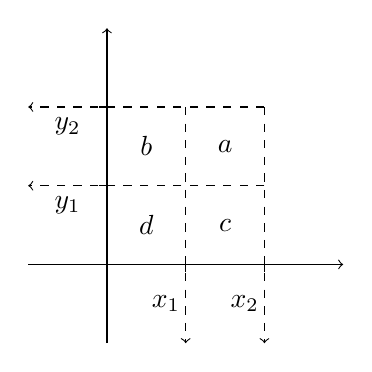
\begin{tikzpicture}
                        \node at (1.5, 1.5) {$a$};
                        \node at (0.5, 1.5) {$b$};
                        \node at (1.5, 0.5) {$c$};
                        \node at (0.5, 0.5) {$d$};
                        \node at (0.75, -0.5) {$x_1$};
                        \node at (1.75, -0.5) {$x_2$};
                        \node at (-0.5, 0.75) {$y_1$};
                        \node at (-0.5, 1.75) {$y_2$};
                        \draw
                        (1, -0.1) -- (1, 0.1)
                        (2, -0.1) -- (2, 0.1)
                        (-1, 0) edge[->] (3, 0)
                        (-0.1, 1) -- (0.1, 1)
                        (-0.1, 2) -- (0.1, 2)
                        (0, -1) edge[->] (0, 3);
                        \draw[dashed]
                        (2, 2) edge[->] (-1, 2)
                        (2, 2) edge[->] (2, -1)
                        (2, 1) edge[->] (-1, 1)
                        (1, 2) edge[->] (1, -1);
                    \end{tikzpicture}
                \end{center}
            \subsubsection*{Joint Probability Mass Function}
                If $X$ and $Y$ are both discrete random variables, we can define the joint probability mass function (for $x, y \in \mathbb{R}$) as;
                \begin{center}
                    $p_{XY}(x, y) = P_{XY}(X = x, Y = y)$
                \end{center}
                And recover the marginal probability mass functions $p_X$ and $p_Y$ by the law of total probability;
                \begin{itemize}
                    \itemsep0em
                    \item $p_X(x) = \summation{y}{} p_{XY}(x, y)$ \hfill $\forall x \in \mathbb{R}$
                    \item $p_Y(y) = \summation{x}{} p_{XY}(x, y)$ \hfill $\forall y \in \mathbb{R}$
                \end{itemize}
                Similarly, for $p_{XY}$ to be valid, the following conditions must hold;
                \begin{itemize}
                    \itemsep0em
                    \item $0 \leq p_{XY}(x, y) \leq 1$, $\forall x, y \in \mathbb{R}$
                    \item $\summation{y}{} \summation{x}{} p_{XY}(x, y) = 1$
                \end{itemize}
            \subsubsection*{Joint Probability Density Function}
                On the other hand, we say $X$ and $Y$ are \textbf{jointly continuous} if there exists a \textbf{joint probability density function} $f_{XY} : \mathbb{R} \times \mat{R} \to \mathbb{R}$, such that the following holds ($B_{XY} \subseteq \mathbb{R} \times \mathbb{R}$);
                $$P_{XY}(B_{XY}) = \defint{(x, y) \in B_{XY}}{}{f_{XY}(x, y)}{x\mathrm{d}y}$$
                We can then define the \textbf{joint cumulative distribution function} $F_{XY}$, for $x, y \in \mathbb{R}$ as;
                $$F_{XY}(x, y) = \defint{t = -\infty}{t = y}{\defint{s = -\infty}{s = x}{f_{XY}(s, t)}{s}}{t}$$
                The joint probability density function can be identified as follows;
                $$f_{XY}(x, y) = \pdif{^2}{x\partial y}F_{XY}(x, y)$$
                The marginal densities $f_X$ and $f_Y$ can be obtained as follows;
                \begin{align*}
                    f_X(x) & = \dif{}{x}F_X(x) \\
                    & = \dif{}{x}F_{XY}(x, \infty) \\
                    & = \dif{}{x} \defint{y = -\infty}{y = \infty}{\defint{s = -\infty}{s = x}{f_{XY}(s, y)}{s}}{y} \\
                    & = \defint{y = -\infty}{y = \infty}{f_{XY}(x, y)}{y} \\
                    f_Y(y) & = \dif{}{y} \defint{x = -\infty}{x = \infty}{\defint{s = -\infty}{s = y}{f_{XY}(x, s)}{s}}{x} \\
                    & = \defint{x = -\infty}{x = \infty}{f_{XY}(x, y)}{x} \\
                \end{align*}
                Similarly, for $f_{XY}$ to be valid, the following conditions must hold;
                \begin{itemize}
                    \itemsep0em
                    \item $f_{XY}(x, y) \geq 0$, $\forall x, y \in \mathbb{R}$
                    \item $\defint{y = -\infty}{y = \infty}{\defint{x = -\infty}{x = \infty}{f_{XY}(x, y)}{x}}{y} = 1$
                \end{itemize}
            \subsubsection*{Independence of Random Variables and Conditional Distributions}
                Two random variables $X, Y$ are independent if, and only if, $\forall B_X, B_Y \subseteq \mathbb{R}$;
                \begin{center}
                    $P_{XY}(B_X, B_Y) = P_X(B_X) P_Y(B_Y)$
                \end{center}
                Or more specifically, $\forall x, y \in \mathbb{R}$;
                \begin{itemize}
                    \itemsep0em
                    \item \textbf{discrete} \hfill $p_{XY}(x, y) = p_X(x) p_Y(y)$
                    \item \textbf{continuous} \hfill $f_{XY}(x, y) = f_X(x) f_Y(y)$
                \end{itemize}
                We define the conditional probability distribution $P_{Y|X}$, for $B_X, B_Y \subseteq \mathbb{R}$ as follows;
                $$P_{Y|X}(B_Y|B_X) = \frac{P_{XY}(B_X, B_Y)}{P_X(B_X)}$$
                Which is the revised probability of $Y$ falling in $B_Y$, given we know $X \in B_X$.
                Therefore, $X$ and $Y$ are independent if, and only if, $P_{Y|X}(B_Y|B_X) = P_Y(B_Y)$, $\forall B_X, B_Y \subseteq \mathbb{R}$.
                Or more specifically, $\forall x, y \in \mathbb{R}$;
                \begin{itemize}
                    \itemsep0em
                    \item \textbf{discrete} \hfill $p_{Y|X}(y|x) = \frac{p_{XY}(x, y)}{p_X(x)}$
                    \item \textbf{continuous} \hfill $f_{Y|X}(y|x) = \frac{f_{XY}(x, y)}{f_X(x)}$
                \end{itemize}
                Similarly, $X$ and $Y$ are independent if, and only, if $p_{Y|X}(y|x) = p_Y(y)$ or $f_{Y|X}(y|x) = f_Y(y)$, $\forall x, y \in \mathbb{R}$.
                \medskip

                We can also define the partition rule as follows;
                \begin{itemize}
                    \itemsep0em
                    \item \textbf{discrete}
                        $$p_X(x) = \summation{y}{} p_{X|Y}(x|y) p_Y(y)$$
                    \item \textbf{continuous}
                        $$f_X(x) = \defint{y = -\infty}{\infty}{f_{X|Y}(x|y)f_Y(y)}{y} \text{ \textbf{and also} } F_X(x) = \defint{y = -\infty}{\infty}{F_{X|Y}(x|y)f_Y(y)}{y}$$
                \end{itemize}
        \subsection*{13th February 2020}
            \subsubsection*{Expectation of a Function of Random Variables}
                Let $g : \mathbb{R} \times \mathbb{R} \to \mathbb{R}$ be a bivariate function of the random variables $X$ and $Y$.
                We define the expectations as follows;
                \begin{itemize}
                    \itemsep0em
                    \item \textbf{discrete}
                        $$E_{XY}(g(X, Y)) = \summation{y}{} \summation{x}{} g(x, y)p_{XY}(x, y)$$
                    \item \textbf{continuous}
                        $$E_{XY}(g(X, Y)) = \defint{y = -\infty}{y = \infty}{\defint{x = -\infty}{x = \infty}{g(x, y)f_{XY}(x, y)}{x}}{y}$$
                \end{itemize}
                From these definitions, we have the following;
                \begin{itemize}
                    \itemsep0em
                    \item if $g(X, Y) = g_1(X) + g_2(Y)$; \hfill $E_{XY}(g_1(X) + g_2(Y)) = E_X(g_1(X)) + E_Y(g_2(Y))$
                    \item if $g(X, Y) = g_1(X)g_2(Y)$ and $X, Y$ independent \hfill $E_{XY}(g_1(X)g_2(Y)) = E_X(g_1(X))E_Y(g_2(Y))$
                    \item if $g(X, Y) = XY$ and $X, Y$ independent \hfill $E_{XY}(XY) = E_X(X)E_Y(Y)$
                \end{itemize}
                The conditional expectation of a random variable $Y$, given that a random variable $X = x$ is;
                \begin{itemize}
                    \itemsep0em
                    \item \textbf{discrete}
                        $$E_{Y|X}(Y|x) = \summation{y}{} yp_{Y|X}(y|x)$$
                    \item \textbf{continuous}
                        $$E_{Y|X}(Y|x) = \defint{y = -\infty}{\infty}{yf_{Y|X}(y|x)}{y}$$
                \end{itemize}
                In either case, the conditional expectation is a function of $x$, and not of the random variable $Y$.
                \medskip

                Note that we can also define a random variable as follows;
                \begin{center}
                    $Z = E_{Y|X}(Y|X)$ where $Z(s) = E_{Y|X}(Y|X(s))$
                \end{center}
                This then gives us;
                \begin{center}
                    $E_Y(Y) = E_X(E_{Y|X}(Y|X))$
                \end{center}
                I hope the tower rule is not examinable.
            \subsubsection*{Covariance and Correlation}
                For a single random variable $X$, we considered the expectation of $g(X) = (X - \mu_X)(X - \mu_X)$ as the variance, and denoted it $\sigma_X^2$.
                The extension of this, to two variables, is the expectation of $g(X, Y) = (X - \mu_X)(Y - \mu_Y)$, which we denote the \textbf{covariance}, $\sigma_{XY}$.
                \begin{align*}
                    \sigma_{XY} & = \text{Cov}(X, Y) \\
                    & = E_{XY}((X - \mu_X)(Y - \mu_Y)) \\
                    & = E_{XY}(XY) - \mu_X\mu_Y
                \end{align*}
                Note that for \textbf{independent} random variables, $E_{XY}(XY) = E_X(X)E_Y(Y) = \mu_X\mu_Y$, therefore $\sigma_{XY} = 0$.
                This measures how two random variables change in tandem with one another.
                \medskip

                This is closely related to the idea of correlation, and therefore the correlation of $X$ and $Y$ can be defined as;
                $$\rho_{XY} = \text{Cor}(X, Y) = \frac{\sigma_{XY}}{\sigma_X\sigma_Y}$$
                This is invariant to the scale of the random variables (and therefore lies between -1 and 1).
                Additionally, if $X$ and $Y$ are independent, then $\sigma_{XY} = \rho_{XY} = 0$ (does not necessarily apply the other way around).
            \subsubsection*{Example Questions}
                \begin{enumerate}[1.]
                    \itemsep0em
                    \item a
                        Let $X, Y$ be independent exponential random variables with parameters $\lambda, \mu$ respectively.
                        What is the probability $X < Y$?
                        \begin{enumerate}[{s}1:]
                            \itemsep0em
                            \item direct
                                \begin{align*}
                                    P(X < Y) & = \defint{x < y}{}{f_{XY}(x, y)}{x\mathrm{d}y} \\
                                    & = \defint{y = -\infty}{y = \infty}{\defint{x = -\infty}{x = y}{f_{XY}(x, y)}{x}}{y} \\
                                    & = \defint{y = -\infty}{y = \infty}{\defint{x = -\infty}{x = y}{f_X(x)f_Y(y)}{x}}{y} & \text{by independence} \\
                                    & = \defint{y = -\infty}{y = \infty}{f_Y(y) \defint{x = -\infty}{x = y}{f_X(x)}{x}}{y} & f_Y(y) \text{ is constant w.r.t $x$} \\
                                    & = \defint{y = -\infty}{y = \infty}{F_X(y) f_Y(y)}{y} & \text{by definition of cdf} \\
                                    & = \defint{0}{\infty}{(1 - e^{-\lambda y}) \mu e^{-\mu y}}{y} \\
                                    & = \intbracket{0}{\infty}{-e^{-\mu y}} - \intbracket{0}{\infty}{-\frac{\mu}{\mu + \lambda}e^{-(\mu + \lambda)y}} \\
                                    & = 1 - \frac{\mu}{\mu + \lambda} \\
                                    & = \frac{\lambda}{\mu + \lambda}
                                \end{align*}
                            \item intuition (with partition rule)
                                \begin{align*}
                                    P(X < Y) & = \defint{y = -\infty}{y = \infty}{\defint{x = -\infty}{x = y}{f_{XY}(x, y)}{x}}{y} \\
                                    & = \defint{y = -\infty}{y = \infty}{\defint{x = -\infty}{x = y}{f_{X|Y}(x|y) f_Y(y)}{x}}{y} \\
                                    & = \defint{y = -\infty}{y = \infty}{F_{X|Y}(y|y) f_Y(y)}{y} & \text{intuition here} \\
                                    & = \defint{y = -\infty}{y = \infty}{F_X(y) f_Y(y)}{y} & \text{by independence} \\
                                    & = \cdots
                                \end{align*}
                        \end{enumerate}
                    \item
                        Suppose that the lifetime, $X$, and brightness, $Y$, of a light bulb are modelled as continuous random variables.
                        Let their joint probability distribution function be given by;
                        \begin{center}
                            $f(x, y) = \lambda_1\lambda_2e^{-\lambda_1 x - \lambda_2 y}$ for $x, y > 0$
                        \end{center}
                        Are lifetime and brightness independent?
                        \begin{align*}
                            f_X(x) & = \defint{-\infty}{\infty}{f(x, y)}{y} \\
                            & = \defint{-\infty}{\infty}{\lambda_1\lambda_2e^{-\lambda_1 x - \lambda_2 y}}{y} \\
                            & = \defint{-\infty}{\infty}{\lambda_1 e^{-\lambda_1 x} \lambda_2 e^{-\lambda_2 y}}{y} \\
                            & = \lambda_1 e^{-\lambda_1 x} \defint{-\infty}{\infty}{\lambda_2 e^{-\lambda_2 y}}{y} \\
                            & = \lambda_1 e^{-\lambda_1 x} & \text{note it is a pdf, hence integrates to 1} \\
                            f_Y(y) & = \lambda_2 e^{-\lambda_2 y} & \text{same as above} \\
                            f_{XY}(x, y) & = f_X(x)f_Y(y)
                        \end{align*}
                        Hence $X$ and $Y$ are independent.
                    \item Suppose continuous random variables $(X, Y) \in \mathbb{R}^2$ have joint probability density function
                        $$f(x, y) = \begin{cases}
                            1 & | x | + | y | < \frac{1}{\sqrt{2}} \\
                            0 & \text{otherwise}
                        \end{cases}$$
                        Determine the marginal probability density functions for $X$ and $Y$.
                        \medskip

                        First determine the range of values for $y$;
                        $$| x | + | y | < \frac{1}{\sqrt{2}} \Leftrightarrow | y | < \frac{1}{\sqrt{2}} - | x | \Leftrightarrow  -\left(\frac{1}{\sqrt{2}} - | x |\right) < y < \frac{1}{\sqrt{2}} - | x |$$
                        \begin{align*}
                            f_X(x) & = \defint{y = -\infty}{y = \infty}{f(x, y)}{y} \\
                            & = \defint{y = -\left(\frac{1}{\sqrt{2}} - | x |\right)}{y = \frac{1}{\sqrt{2}} - | x |}{1}{y} \\
                            & = \sqrt{2} - 2| x | \\
                            f_Y(y) & = \sqrt{2} - 2| y | & \text{same as above}
                        \end{align*}
                        Hence $f_X(x)f_Y(y) \neq f_{XY}(x, y)$, therefore $X$ and $Y$ are not independent.
                \end{enumerate}
 \end{document}